\section{Approach}
The new \texttt{vtkGPUVolumeRayCastMapper} uses a ray casting
technique\cite{hadwiger_real-time_2006} for volume rendering which is a
state-of-the-art for volume rendering on modern graphics platforms.
Algorithmically, at a high level, it is similar to the older version of this
class (although with a fairly different OpenGL implementation since that
original class was first written over a decade ago and used GPU assembly code).
One of the main reason we chose to use ray casting due to the flexibility of
this technique, which enables us to support all the features of the software ray
cast mapper but with the acceleration of the GPU. Ray casting is an image-order
rendering technique, with one or more rays cast through the volume per image
pixel. VTK is inherently an object-order rendering system, where the GPU renders
all graphical primitives (points, lines, triangles, etc.) represented by
vtkProp(s) in the scene in one or more passes (with multiple passes needed to
support advanced features such as depth peeling for transparency).

The image-order rendering process for vtkVolume is initiated when the
front-facing polygons of the volume’s bounding box are rendered with a custom
fragment program. This fragment program is used to cast a ray through the volume
at each pixel, with the fragment location indicating the starting location for
that ray. The volume and all the various rendering parameters are transferred to
the GPU through the use of textures (3D for the volume, 1D for the various
transfer functions) and uniform variables. Steps are taken along the ray until
the ray exits the volume, and the resulting computed color and opacity are
blended into the current pixel value. Note that volumes are rendered after all
opaque geometry in the scene to allow the ray casting process to terminate at
the depth value stored in the depth buffer for that pixel (and, hence, correctly
intermix with opaque geometry).

In addition to providing supported features of the old mapper, the new mapper
added new capabilities such as clipping on GPU,  gradient opacity, and volume
picking amongst many others. In the next few sections, we will cover each of
these features in detail.

\subsection{Single Pass}
\begin{figure}[h]
  \centering
  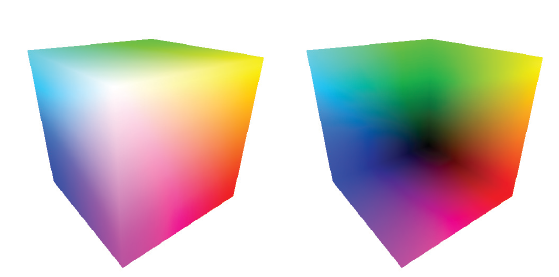
\includegraphics[width=\columnwidth]{frontandback.png}
  \caption{Front and back faces are rendered for start and end position of the
  ray.}
  \label{fig:frontandback}
\end{figure}%


\begin{figure}[h]
  \centering
  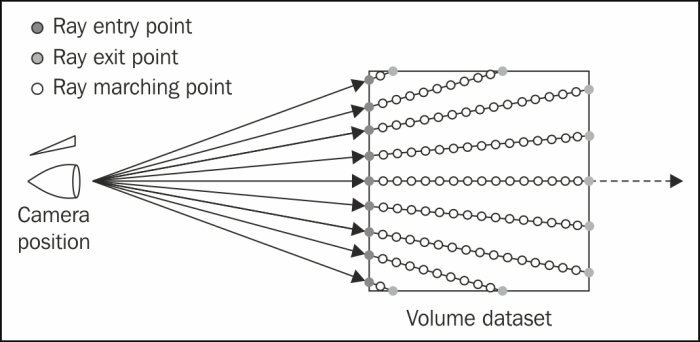
\includegraphics[width=\columnwidth]{raycasting.jpg}
  \caption{Implementing volume rendering using single-pass GPU ray casting.}
  \label{fig:raycasting}
\end{figure}%

In a ray-casting algorithm, the entry and the exit point into the volume is
needed to determine when to stop the ray-marching. To determine the entry and
the exit point, one approach is to render the geometry of the volume bounding
box of the volume twice. In the first pass, the front face of the geometry is
rendered and in the second pass the backface is rendered as shown in
Figure~\ref{fig:frontandback}. Using the interpolated vertex position and
texture lookup, the start and end positions is computed. Instead of this, in
\texttt{vtkGPUVolumeRayCastMapper}, entry and exit points are computed based on
the fact that the texture extents of the volume is within vec3(1.0), vec3(-1.0)
range (as shown in Figure~\ref{fig:raycasting}). The code below is showing the
fragment shader piece that determines whether or not to stop marching the rays
depending on the value of stop.
 
 \begin{lstlisting}[breaklines=true]
 bool stop = any(greaterThan(g_dataPos, 
                 ip_texMax)) ||
             any(lessThan(g_dataPos, 
                 ip_texMin));
 \end{lstlisting}
 
 The advantage of such approach is that it requires one less pass and is faster than other approaches since there is no texture generation or lookup happens for determining the termination of the ray.
 
 
\subsection{Dynamic Shader Generation}
In the new \texttt{vtkOpenGLGPUVolumeRayCastMapper} all the operations are
performed on the GPU. The advantage of this approach was a more streamlined code
that is easier to maintain and debug. This approach also provided an opportunity
to rework how to support different features without having too many branches in
the shader code or having to send all the options to the shader because that
would have been detrimental to the performance. In the new
\texttt{vtkOpenGLGPUVolumeRayCastMapper}, the shader is dynamically composed by
the mapper. For this to work, we have introduced tags in a vertex or fragment
shader which are then replaced by the \texttt{vtkShaderComposer} depending on
the options enabled or chosen by the application code. For instance, the
skeleton fragment shader defines tags as shown below:
 
 \begin{lstlisting}
//VTK::Base::Dec

//VTK::Termination::Dec 
\end{lstlisting}

At the run time then \texttt{//VTK::Base::Dec} is then replaced by the code
shown below. 

To define a structure, we have chosen a strategy that separates the tags in
found category: 

\begin{enumerate}
  \item Declaration (::Dec) The tags belong to this group are meant to declare
    variables or function outside the main execution of the shader code. The
    variables defined are uniform, varying, and user-defined global variables.
    The functions defined are typically perform operations that are repetitive
    in nature such as computing color of a fragment. 

  \item Initialization (::Init) The tags belong to this group are meant to
    initialize variables inside the main execution function of the shader but
    before the ray-casting loop in the fragment shader. An example of such code
    includes computation of the initial position of ray and direction of ray
    traversal.

  \item Implementation (::Impl) The tags belong to this group are the variables
    or functions or the combination of both that perform the actual operation of
    clipping, cropping, shading, etc. on one, two, or four component volume
    data.  The implementation code used local and global variables and optimized
    for performance reasons as they are executed as long as the ray is
    traversing inside the volume and didn't run into a termination condition
    which is checked every time.  

  \item Exit (::Exit) The tags belong to this group perform final computation
    such as the final color of the fragment. These tags are placed outside the
    ray-casting loop and typically contain numeric assignments. 
\end{enumerate}

\subsection{Lighting / Shading}
The old mapper supported only one light (due to limitations in OpenGL at the
time the class was written). The \texttt{vtkFixedPointVolumeRayCastMapper}
supports multiple lights, but only with an approximate lighting model, since
gradients are precomputed and quantized, and shading is performed for each
potential gradient direction regardless of fragment location. The new mapper
accurately implemented the VTK lighting model to produce high quality images for
publication. To support this, depending on the light type (point, directional,
and positional), the lighting parameters are sent to the shader which then
performs the per pixel lighting calculations. The number of lights is limited to
six mostly for performance reasons as the interactive frame rate goes down
significantly with each light added to the scene. The Phong shading lighting
model is used for volume rendering lighting. Phong lighting requires normals
which have to be computed for each fragment. The normal calculation is done by
first computing the gradient and then scaling the gradient by the spacing
between the cells. The gradient is computed by reading the scalar values form
the neighboring cdells using the offset vector that stores the step size based
on the bounds of the volume. 

\subsection{Volume Picking}
Picking, in the context of volume rendering, is
the action of resolving the set of voxels a user has clicked on with the
pointer. This provides the user with means to interact with the objects in a 3D
scene. VTK legacy volume mappers support picking through an instance external to
the mapper itself called ~\texttt{vtkVolumePicker}.  This class casts a ray into
the volume and returns the point where the ray intersects an isosurface of a
user specified opacity. This technique has certain limitations given that the
picking class does not have enough information to correctly account for
clipping, transfer functions and other parameters defining how the mapper
actually renders, thus reducing its reliability on the actual objects being
picked.

VTK supports hardware-accelerated picking of goemetric data through the class
~\texttt{vtkHardwareSelector}, which uses a multiple-render-pass approach in
order to resolve the various objects in a scene (actors in VTK parlance) and
their corresponding primitives.  Each pass renders separately a different
selection abstraction ( processes, actors, composite blocks and primitives),
painting with a different color each of the various components in the scene.
The images rendered by each pass are downloaded from the GPU and subsequently
analyzed in the class thereby resolving the correspondence of each pixel to its
particular actor, primitive, etc.

The inherent flexibility of the revamped shader implementation of this mapper
permits a seamless integration with ~\texttt{vtkHardwareSelector}'s interface by
rendering the appropriate colors for each of its passes, hence granting
consistency in the object selection regardless of whether it is geometric or
volumetric data.  Providing selection support directly within the fragment
shader ensures high selection accuracy even in situations where a volume
intermixes with geometry in seemingly cumbersome ways or other advanced features
(e.g. clipping) are enabled (what you see is what you pick).  Given the readily
available picking styles supported by ~\texttt{vtkHardwareSelector} (e.g.
~\texttt{vtkAreaPicker}), it is possible to make a selection of a specific set
of visible voxels.

\subsection{Volume Texture Streaming} An intrinsic limitation of volume
rendering is that the 3D volume data to be rendered does not always fit into the
graphics memory of a system. Such limitation becomes increasingly important to
address now that the new mapper provides support for mobile architectures.  A
relatively simple method when dealing with a large volume is the volume
streaming approach also commonly known as bricking in which the volume is split
into several blocks so that a single sub-block (brick) fits completely into GPU
memory.  Each sub-block is stored in main memory and streamed into GPU memory
for a rendering pass one at a time (in a back-to-front manner for correct
composition). The sub-blocks are rendered using the standard shader programs and
alpha-blended with each other by OpenGL. Streaming the volume as separate
texture bricks certainly, imposes a performance trade-off but acts as a graphics
memory expansion scheme for devices that would not be able to render a higher
quality volume otherwise.

\subsection{Dual Depth-Peeling}
VTK has long supported the use of depth-peeling for order-independent rendering
of translucent geometry. Since translucent fragments must be blended in a
specific order to obtain the correct pixel color, techniques like depth-peeling
are necessary for correctly shading a complex scene.

In a multipass depth-peeling rendering, `slices' of fragments are pulled from
the scene in depth order; first the nearest fragments per pixel are collected in
the first pass, and then the fragments just behind those are written in the next
pass. After each pass, the current set of fragments is blended into an
accumulation buffer, ultimately producing a correctly colored scene in which all
fragments are blended from front-to-back.

The standard depth-peeling algorithm, which collects a single layer of fragments
per geometry pass in front-to-back order, was recently updated to use a ``dual
depth-peeling'' technique\cite{bavoil_order_2008}, in which two layers of
fragments are peeled in a single geometry pass: One layer from the front and a
second from the back. These are blended into two separate accumulation buffers
and eventually the front and back peels will meet towards the middle of the
geometry. This allows depth-peeling to be carried out in roughly half as many
geometry passes.

An interesting detail of the new depth-peeling implementation is that there are
four depth values available per-pixel during a typical peeling pass. Two depth
values each are associated with the front and back peels; these are the depth of
the currently peeled fragment, and the depth of the next fragment that will be
peeled. These depth values can be reinterpreted as two sets of ``inner'' and
``outer'' boundaries for a view-ray traversing a volume.

By adapting the volume mapper's fragment shader to use these depth values for
computing two ``slices'' of a volume, we are able to integrate volume rendering
into our depth-peeling pass. This enables volumetric data to be mixed with
translucent geometry while efficiently yielding a correctly colored result.
 
\subsection{Render to texture}
Typically, the mapper uses a single pass
rendering approach in which the 3D volume data is rendered on screen i.e. the
default framebuffer that comprises of a color and a depth buffer. In games and
other graphics applications, a multi-pass rendering approach called ``Render to
Texture'' is used to support advanced visual rendering techniques such as
deferred shading, texture baking, post processing, etc. This technique uses the
rendered output from one pass to modify/enhance the output of another rendering
passes. 

\begin{figure}[h]
\centering
  \begin{subfigure}[b]{.5\columnwidth}
    \centering
    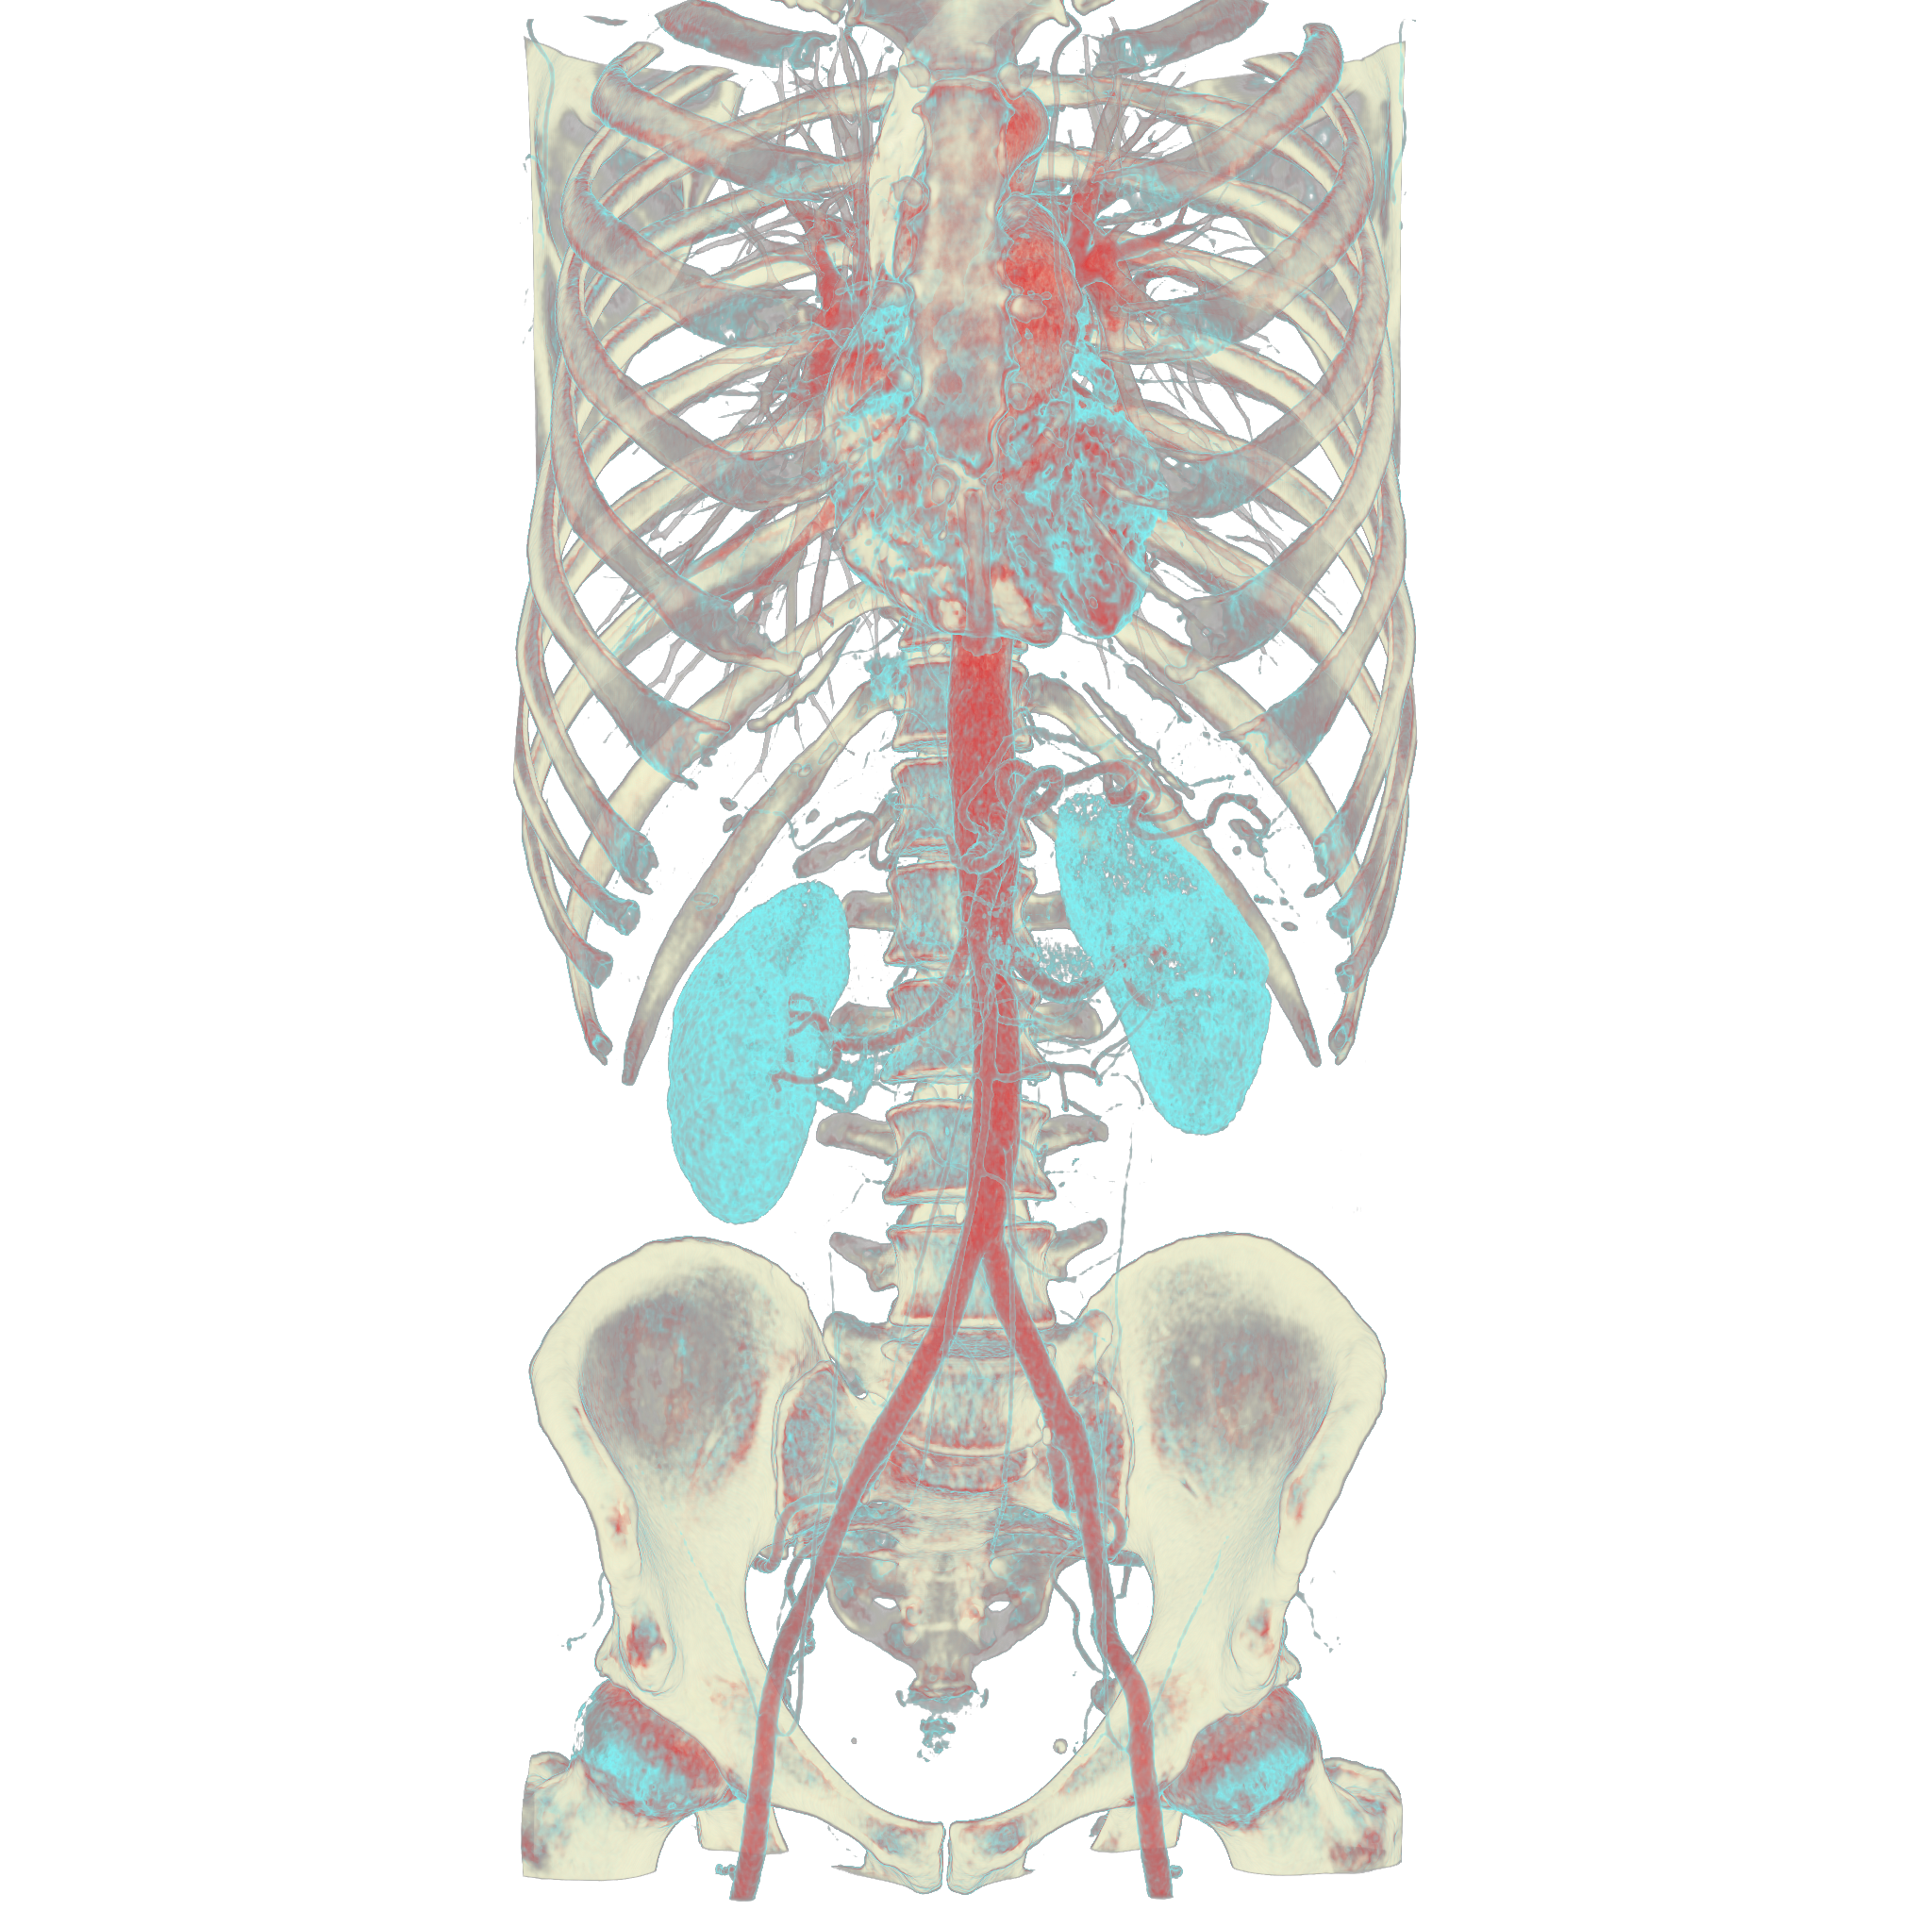
\includegraphics[width=\textwidth]{colorimage.png}
    \caption{Color image}
    \label{fig:rendertotexturecolor}
  \end{subfigure}%
  \begin{subfigure}[b]{.5\columnwidth}
    \centering
    
\includegraphics[width=\textwidth]{depthimage.png}
    \caption{Depth image}
    \label{fig:rendertotexturedepth}
  \end{subfigure}
  \caption{Render to texture}
  \label{fig:rendertotexture}
\end{figure}

When the \texttt{RenderToImage} flag is enabled, the volume mapper switches
rendering to an OpenGL FrameBufferObject (FBO) and allows the user to obtain the
rendered pixel data via simple image retrieval calls. The mapper provides
methods to grab color and depth information either as individual textures or as
VTK's image data structure - \texttt{vtkImageData}. The color data is simply the
pixel representation of the rendered volume whereas depth data consists of a
grayscale image depicting how deep each voxel is in the scene. When an
application enables render to texture mode, a framebuffer object is created, the
vertex and fragment shader are generated, color and depth buffers are cleared,
and the color is set to white with a value of zero alpha. The value of zero
alpha is used so that applications can safely ignore the transparent pixels and
the color buffer is set to white color because white represents the maximum
depth, that is the depth of the far plane. In the render to texture pass, the
fragment shader writes to color and depth target and to write the depth
information it uses the depth of first non-transparent voxel.

\subsection{Mobile Support}
The decision to use OpenGL 3 or higher enabled volume rendering to support
mobile devices (iOS and Android devices) as OpenGL ES 3.0 supports 3D textures.
However the OpenGL ES does not support all of the texture format types, and
therefore, new texture formats are added with compile time switch to enable or
disable them depending on whether the platform is desktop or mobile. One such
example is capturing of depth buffer since that is not yet supported on the
mobile platform.  Since typically interactions on mobile devices require touch
interactions, the new rendering system added support for multiple touch events
such as using two fingers to translate, rotate, and zoom the camera. With minor
feature-set exceptions, the new volume mapper works on mobile devices enabling
developers to build sophisticated applications for the scientific community.

\subsection{Optimizations and Edge-Cases} The new
\texttt{vtkOpenGLGPUVolumeRayCastMapper} is more than just a ray cast mapper
implementation. It is designed to work on multiple platforms and developed to
perform volume rendering at interactive frame rates. To achieve interactive
frame rates and to handle edge cases, we have implemented following
optimizations in the new mapper. 

\begin{itemize}
  \item Clipping plane optimization In VTK a user can place multiple planes at
    desired angles to clip the volume. This technique is essential for many
    medical use-cases. Since only one side of clip planes needs to be traversed,
    performing any sort of ray cast on the clipped side is wasteful. Hence a
    simple optimization is to move the starting point of the ray on the plane by
    projecting the ray onto the plane in the view direction. 

  \item Eye Too Close to the Volume When the eye is too close to the volume, the
    near plane could clip the volume visible bounds resulting in OpenGL clipping
    removing the geometry from rendering. In such cases the bounding box of the
    volume that defines the texture coordinates and hence define a surface to
    start casting the ray needs to be clipped. To handle such scenario, a
    plane-box intersection is added. So far evey move of the camera is funding
    invokved checking if the geomtry of the volume needs to be clipped.

\item Support for Double and Long Long Data Type The current OpenGL API does not
  support 64-bit data types. In order to be able to render volumes of these
    types, the mapper loads the data array slice by slice casting the data
    values to floating-point. This, despite the obvious precision loss, is
    provided to the user as a convenience feature.

\end{itemize}
